
\documentclass[a4paper,12pt]{scrbook}
\usepackage{amsmath,amssymb,amsthm}
\usepackage{fancyvrb}
\usepackage{parskip}
\usepackage{lastpage}
\usepackage{verbatim,boxedminipage,enumitem}
\usepackage{ifthen}
\usepackage{color,graphicx}
\usepackage{pgf}
\usepackage{longtable}
\usepackage{upquote}
%\usepackage[all]{xy}
\usepackage{tobiShell}
\usepackage{tikz}
\usetikzlibrary{automata}
\usetikzlibrary{arrows}
\usepackage{pgf,pgfarrows,pgfnodes}
\usepackage{pgfplots}
\usepackage{circuitikz}
\usetikzlibrary{circuits}
\usetikzlibrary{circuits.logic.US}
\usepackage{mymath}
\usepackage{python}
%------------------------------------------------------------------
% Verbatim for console window - single line frame, no line numbers
%------------------------------------------------------------------
\DefineVerbatimEnvironment%
 {console}{Verbatim}
 {frame=single}

%--------------------------------------------------------
% Remove the vertical spacing before and after Verbatim.
%--------------------------------------------------------
\usepackage{atbeginend}
\BeforeBegin{console}{\mbox{}\\ \begin{minipage}{\textwidth}\vspace{3pt}}
\AfterEnd{console}{\vspace{4pt} \end{minipage} \\ }

\begin{document}
\thispagestyle{empty}

\begin{center}
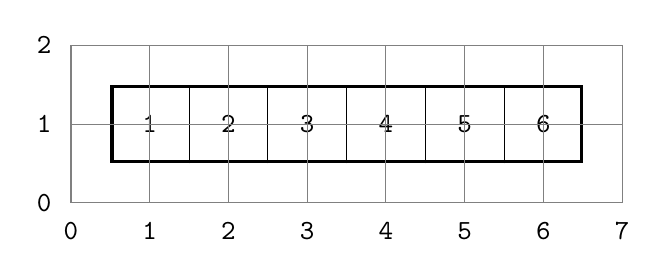
\begin{tikzpicture}

\draw (3.5, 1.0)
  node[draw, line width=0.04cm, , color=black,
       rounded corners=0.0cm, inner sep=0.0cm] {

\begin{minipage}[t][0.96cm]{5.96cm}
\mbox{}

\end{minipage}

};\draw[, font=\ttfamily] (1.0, 1.0) node {1};
\draw[black] (1.5,0.5) -- (1.5,1.5);
\draw[, font=\ttfamily] (2.0, 1.0) node {2};
\draw[black] (2.5,0.5) -- (2.5,1.5);
\draw[, font=\ttfamily] (3.0, 1.0) node {3};
\draw[black] (3.5,0.5) -- (3.5,1.5);
\draw[, font=\ttfamily] (4.0, 1.0) node {4};
\draw[black] (4.5,0.5) -- (4.5,1.5);
\draw[, font=\ttfamily] (5.0, 1.0) node {5};
\draw[black] (5.5,0.5) -- (5.5,1.5);
\draw[, font=\ttfamily] (6.0, 1.0) node {6};
\draw[gray] (0,0) -- (0,2);
\draw[gray] (1,0) -- (1,2);
\draw[gray] (2,0) -- (2,2);
\draw[gray] (3,0) -- (3,2);
\draw[gray] (4,0) -- (4,2);
\draw[gray] (5,0) -- (5,2);
\draw[gray] (6,0) -- (6,2);
\draw[gray] (7,0) -- (7,2);
\draw[gray] (0,0) -- (7,0);
\draw[gray] (0,1) -- (7,1);
\draw[gray] (0,2) -- (7,2);
\draw(0, 0) node [font=\ttfamily, label=below:{\texttt{0}}] {};
\draw(1, 0) node [font=\ttfamily, label=below:{\texttt{1}}] {};
\draw(2, 0) node [font=\ttfamily, label=below:{\texttt{2}}] {};
\draw(3, 0) node [font=\ttfamily, label=below:{\texttt{3}}] {};
\draw(4, 0) node [font=\ttfamily, label=below:{\texttt{4}}] {};
\draw(5, 0) node [font=\ttfamily, label=below:{\texttt{5}}] {};
\draw(6, 0) node [font=\ttfamily, label=below:{\texttt{6}}] {};
\draw(7, 0) node [font=\ttfamily, label=below:{\texttt{7}}] {};
\draw(0, 0) node [font=\ttfamily, label=left:{\texttt{0}}] {};
\draw(0, 1) node [font=\ttfamily, label=left:{\texttt{1}}] {};
\draw(0, 2) node [font=\ttfamily, label=left:{\texttt{2}}] {};
\end{tikzpicture}

\end{center}

\end{document}
